\newpage
\subsection{Design Patterns}

Design pattern are well known solutions for recurring problems. By defining and categorizing patterns, a catalog of patterns can be created for use when building large and complex software systems \cite{gof}. Ghosh \cite{dslsInAction} talks about certain design patterns being industry "best - practices" for DSL development. Over the course of this project, these patterns have been used extensively.
\bigskip

\noindent
There are several benefits of using design patterns. Patterns are known solutions for building software systems. This helps increase maintainability, extensibility and readability of the code base \cite{iceland}.

\subsubsection{Singleton Pattern}
The singleton pattern restricts the instantiation of a class to one object, and provides a global point of access to \cite{gof}. It is used when the developer does not want multiple implementations of the type in heap memory. Pure functions, file - system utilities are some of the methods we can wrap inside Utility objects. In this project, the singleton has been used for re - usable components like regular expression and file system utilities. Scala provides an \textbf{Object} type that implements this pattern without requiring any boilerplate code. An example of this pattern is shown below:

\begin{figure}[H]
  \centering
    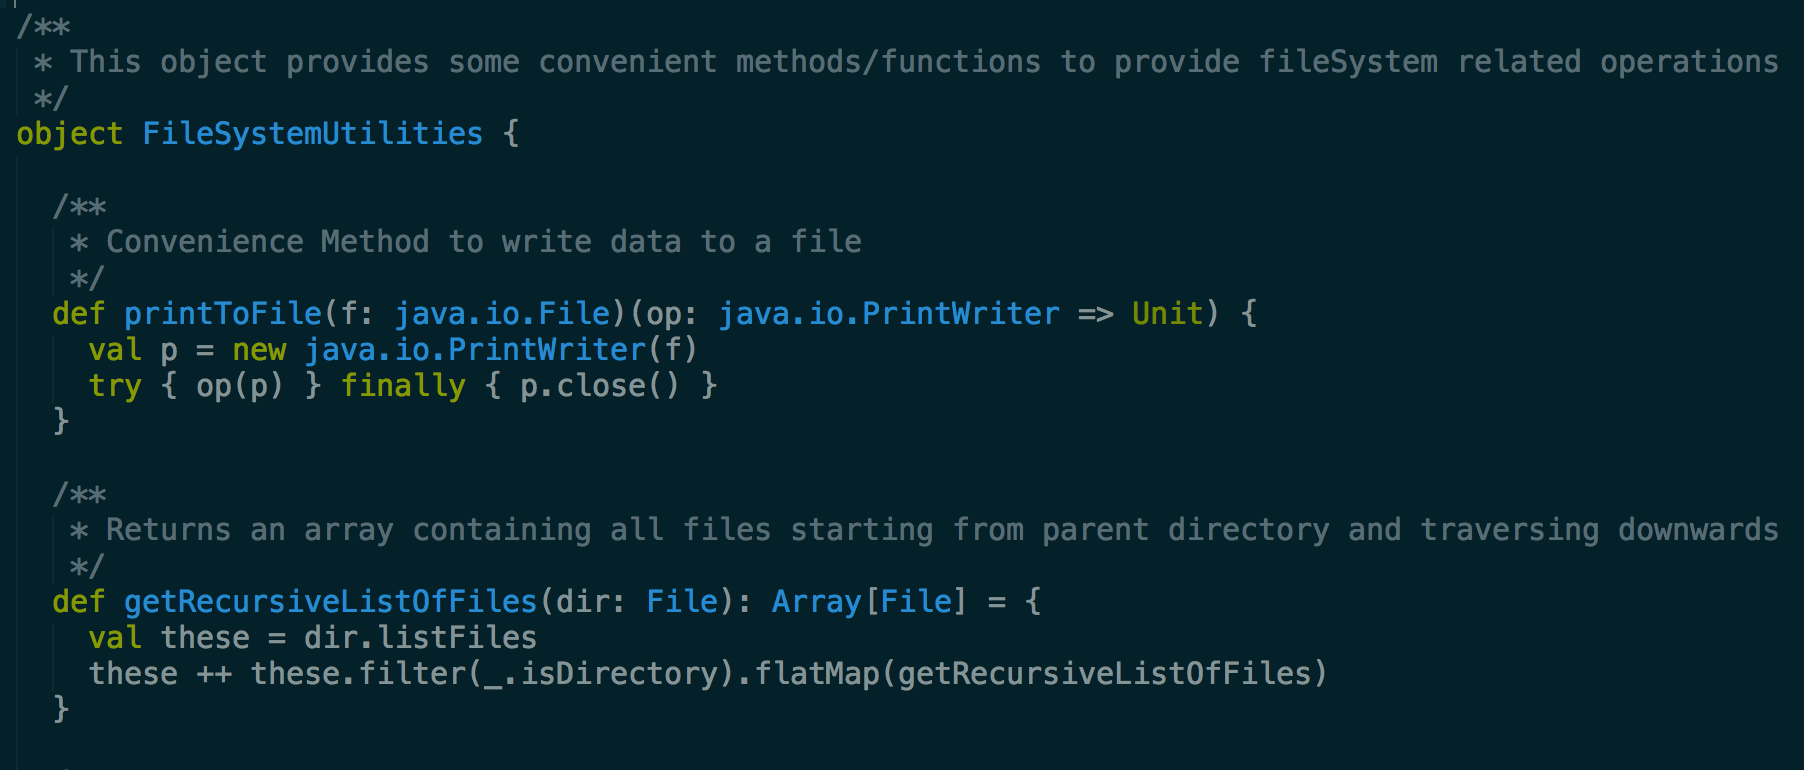
\includegraphics[width=400px]{figures/singleton.png}
  \caption{An example of Singleton pattern usage}
\end{figure}

\noindent
\textbf{Explanation} - The example above is straightforward. The methods inside the object can be directly accessed by invoking \textless object\_name \textgreater.\textless method\_name(args) \textgreater. Scala \textit{objects} also provide a great way to have singleton implementations of traits.
For example, creation of thread - safe methods require an extension of the trait \textbf{Runnable}. Methods can be implemented without considering factors like thread - safety and multiple instantiations.

\begin{figure}[H]
  \centering
    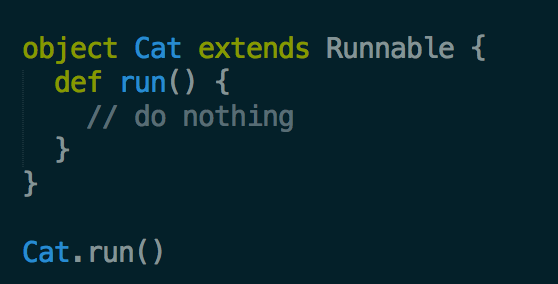
\includegraphics[width=300px]{figures/singleton2.png}
  \caption{An example of Singleton pattern usage}
\end{figure}

\noindent
The reasons for choosing the \textit{Singleton} pattern were:
\begin{itemize}
\item Lazy initialization leading to optimized heap memory usage
\item Concise Syntax
\item Thread Safety
\item Clear Intent
\end{itemize}

% Explanation of Builder Pattern
\subsubsection{Builder Pattern}
Builder pattern builds a complex object using simple objects and using a step by step approach. This type of design pattern comes under creational patterns as this pattern provides one of the best ways to create an object. Our SLEEK/HIP tests are instantiated incrementally and therefore the builder pattern is natural choice. The builder pattern combined with the \textbf{fluent interface} concept gives the DSL a declarative feel.
\bigskip

\noindent
Fowler's concept of the "Fluent Interface" can be extended to Scala which models behaviour using traits rather than interfaces \cite{scala}. This in conjunction with the builder pattern lead to a declarative syntax. One of the uses of the builder is shown below.

\begin{figure}[H]
  \centering
    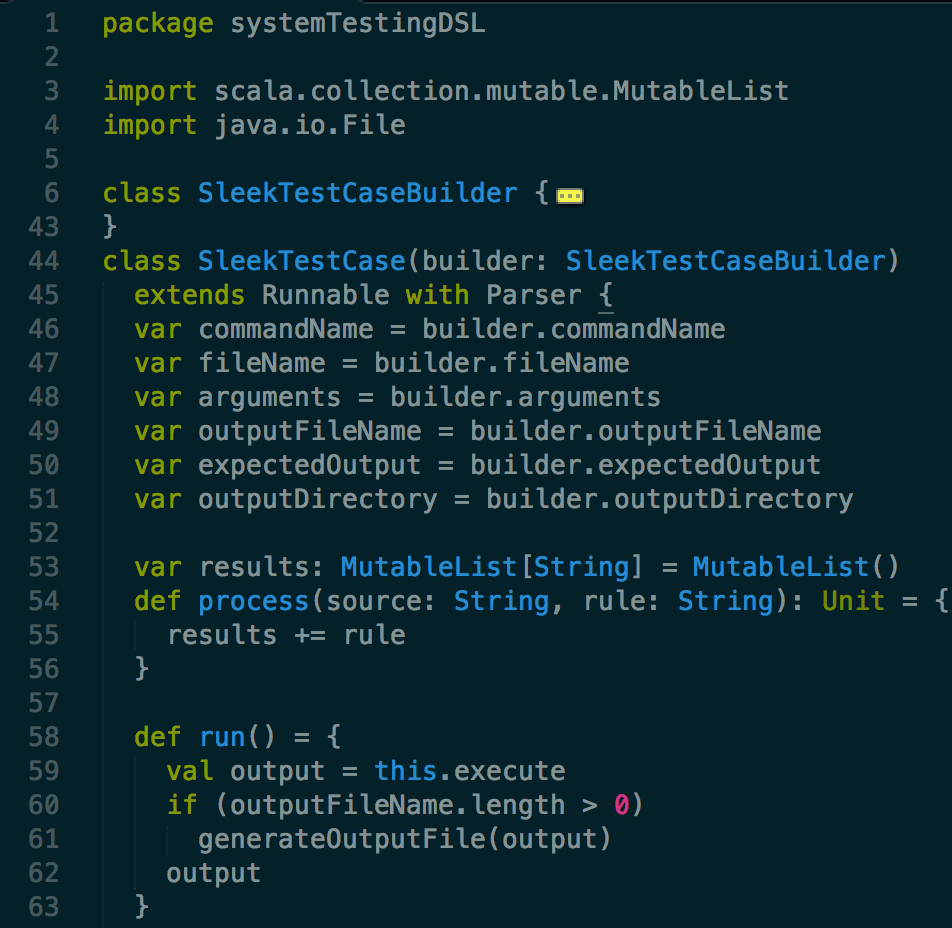
\includegraphics[width=400px]{figures/builder_pattern.png}
  \caption{An example of builder pattern usage}
\end{figure}

\noindent
The reasons for choosing the \textit{Builder} pattern were:
\begin{itemize}
\item Natural language like syntax enhancing readability
\item Logic is built into the syntax
\item The parameters being provided to the base type can be provided in different stages as the builder manages the object instantiation.
\end{itemize}

% Explanation of Factory Pattern
\subsubsection{Factory Pattern}
This is used in the project by defining trait for creating an object, but let the classes that implement the interface decide which class to instantiate. The Factory method lets a class defer instantiation to subclasses. For context - aware choice of which kind of class to instantiate. This has been used to switch between \textbf{Console Output and HTML Output}.

\begin{figure}[H]
  \centering
    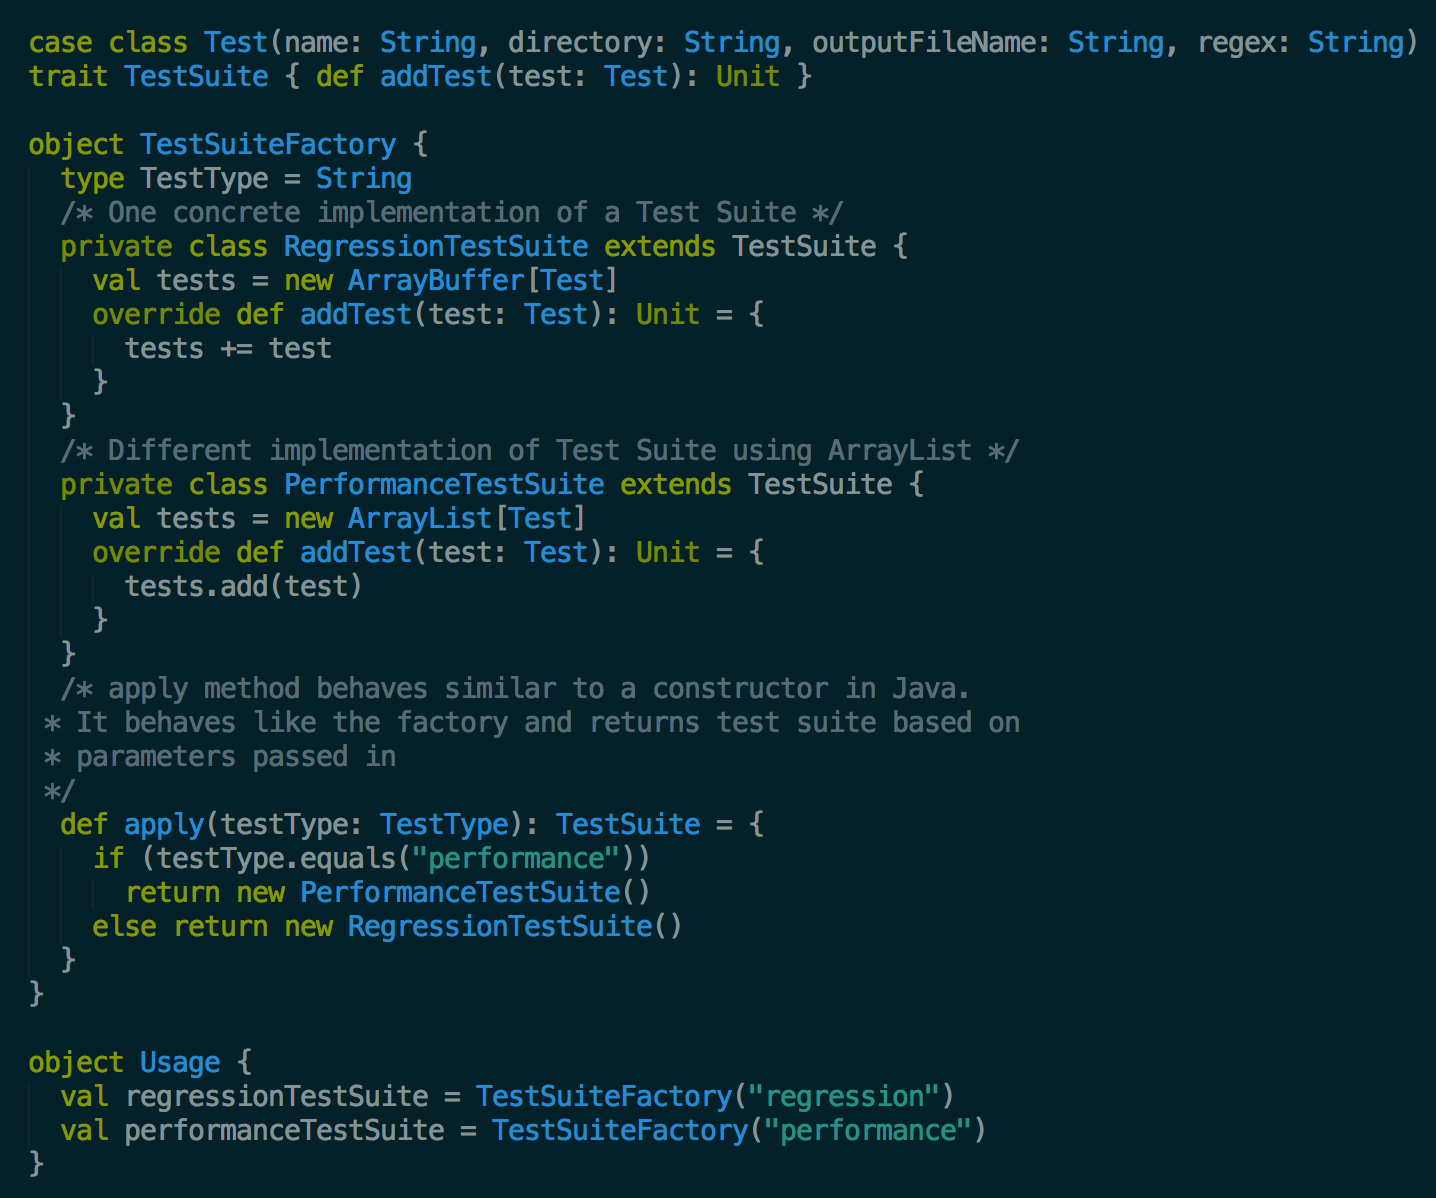
\includegraphics[width=500px]{figures/factory.png}
    \caption{An example of how Factory Pattern is used}
\end{figure}

\noindent
\textbf{Explanation} - The trait \textbf{TestSuite} specifies certain methods that any test suite must implement. Two concrete implementations of \textbf{TestSuite} are \textbf{RegressionTestSuite} and \textbf{PerformanceTestSuite}. The companion object, \textbf{TestSuite} implements the \textbf{Factory Pattern} by deciding which kind of TestSuite to instantiate - the RegressionTestSuite or PerformanceTestSuite based on some input parameters. For the sake of simplicity, here a string type parameter has been shown. However, in the application code, a \textbf{Configuration} type has been passed in as the parameter.

\noindent
The reasons for choosing the \textit{Factory} pattern were:
\begin{itemize}
\item Better abstraction
\item Internal implementation details are not revealed to clients
\item Stronger inheritance relationship
\end{itemize}

% Explanation of Future Timeout
\subsubsection{Future Timeout Design Pattern}
Scala Futures provide an elegant way of handling asynchronous operations in Scala \cite{scala}. They allow developers to write non - blocking processes running on a different thread. They allow us to wait on the thread for completion (which is actually an anti - pattern because we could have just used a blocking call), pass messages/arguments to the thread when it is done executing (\textit{Promises}) or just time - out after a certain duration (\textit{Awaits}). In this context, the time - out pattern using Awaits is being used to prevent processes from blocking indefinitely. This can be set by setting the \textbf{TIMEOUT} variable in the system configuration.

\begin{figure}[H]
  \centering
    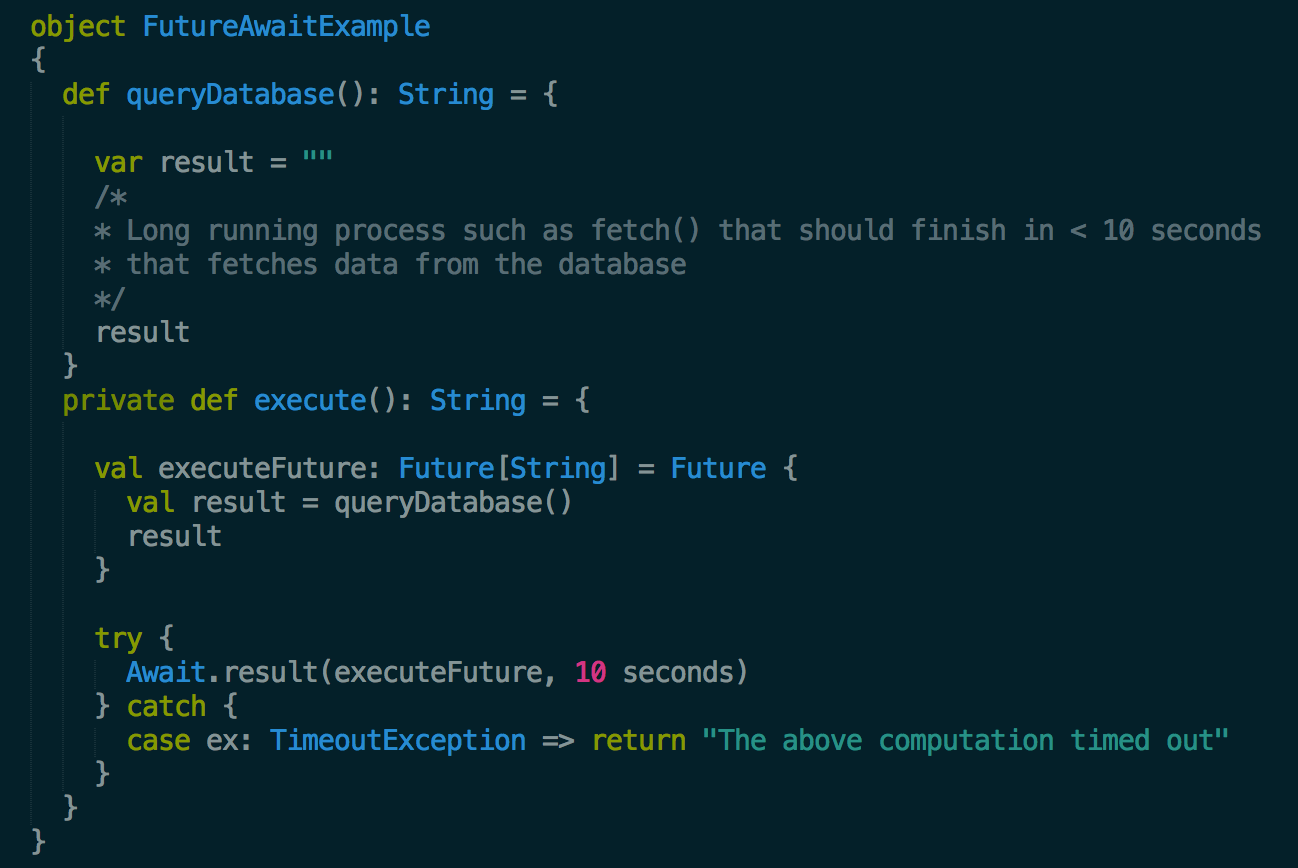
\includegraphics[width=500px]{figures/future_timeout.png}
  \caption{An example of "Future Timeout" pattern usage}
\end{figure}

\noindent
\textbf{Explanation} - The future timeout pattern is specific to languages like Scala that provide concurrent constructs such as \textbf{Futures}, \textbf{Promises} and \textbf{Awaits}. In the above example, the function call that takes a substantial amount of time is the queryDatabase() method, which is supposed to return a \textit{string} value. Scala allows us to wrap it in a \textbf{Future} block. It's return type therefore becomes a \textbf{Future[String]}. The \textbf{Await} construct allows to wait on the Future for a specified time period (in this case 10 seconds). If the computation takes longer, an exception is thrown and dealt with appropriately inside the catch block.

\noindent
The reasons for choosing the \textit{Future - Timeout} pattern were:
\begin{itemize}
\item Concise syntax
\item Logic is built into the syntax
\item Abstracts lower level threading details
\end{itemize}
% Explanation of Dependency Injection
\subsubsection{Dependency Injection (DI) Pattern}

This pattern allows developers to avoid hard-coded dependencies and to substitute dependencies either at run-time or at compile time. It is a special case of the Inversion of Control (IoC) pattern. It also allows us to choose between multiple implementations of a particular component in an application\cite{gof}. DI has been applied throughout the project to reduce coupling and make the code as extensible as possible. For example, \textbf{constructor injection} is performed for configuration type objects where custom configurations are possible.

\begin{figure}[H]
  \centering
    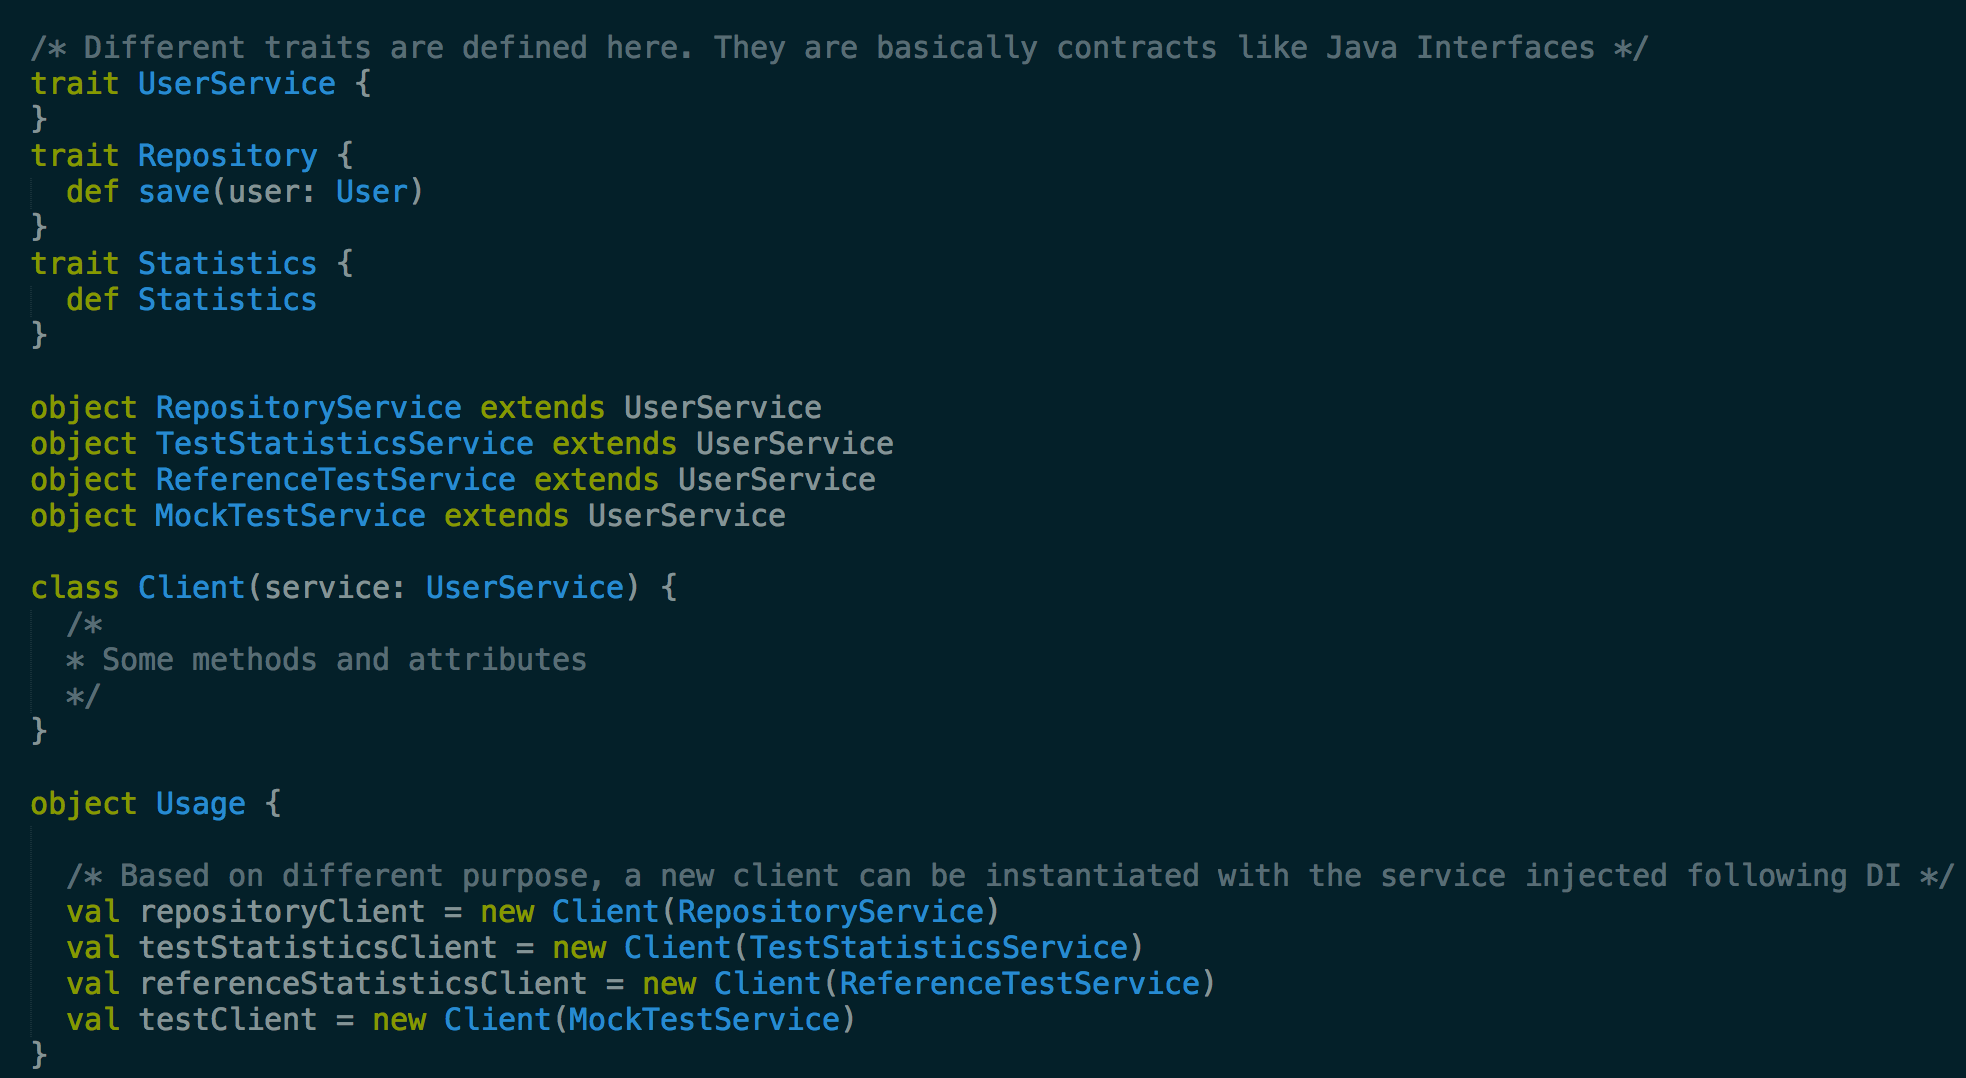
\includegraphics[width=520px]{figures/di.png}
  \caption{An example of how DI is used}
\end{figure}
\noindent

\noindent
\textbf{Explanation}: The DI pattern has been used in several places throughout the project to facilitate ease of testing, multiple implementation support and general loosely coupled design. In the code skeleton above, the \textbf{UserService} trait specifies certain behaviour (like a Java Interface). Some of the concrete implementations of these behaviours are the \textbf{RepositoryService, TestStatisticsService, ReferenceTestService}. The \textbf{MockTestService} is just a drop-in that can be used for unit testing the code. The type Client requires an \textbf{UserService} as a dependency. We can just inject in concrete implementations of the Services based on the kind of Client we are instantiating. This is a simplified example of how DI has been used in the project.
\bigskip

\noindent
The reasons for choosing the \textit{Dependency Injection} pattern were:
\begin{itemize}
\item Loose coupling leading to extensibility
\item Static checking of dependencies (unlike XML based DI implementations)
\item Concise syntax
\end{itemize}